\documentclass[
    headings=optiontohead,              % allows double headers
    12pt,                               % fontsize 
    DIV=13,                             % koma script diveider amount. tells koma how much of the site can be written to
    twoside=false,                      % if set to true, automatically formats as book style with different left and right pages
    open=right,                         % starting page on twosided texts 
    BCOR=00mm,                          % correction that accounts for the center of the pages being glued in
    toc=bibliographynumbered            % bibliography gets a number and is listed in the table of contents
]{scrreport}

\usepackage[english]{babel}                     % font that supports English
\usepackage{upgreek}                            % non-cursive Greek letters
\usepackage[stretch=10,shrink=10,protrusion=true,expansion=true,final]{microtype} % prettier block format
\usepackage{hyperref}                           % links for everything
\usepackage{color}                              % allows for setting in different colors
\usepackage[autooneside=false,automark]{scrlayer-scrpage} % page-style with "Kolumnentitel" (title of current chapter is displayed at the top)
\usepackage{amsfonts,amstext,amsmath,amsthm, amssymb} % better math mode (\mathrm and \text) and symbols
\usepackage[sb]{libertinus}                     % use the font libertinus (needs to be installed from the web)
%\usepackage[slantedGreek]{libertinust1math}     % math mode improvement for libertinus
\usepackage{siunitx}                            % physical units setting
\usepackage{icomma}                             % commas in lists get extra space if needed                        
\usepackage{xspace}                             % works to improve own commands and provides "\xspace"-command, that puts a space if needed
\usepackage{ifthen}                             % more control over non-obligatory parameters
\usepackage{titling}                            % get title values as macros
\usepackage[onehalfspacing]{setspace}           % control the spacing between lines and in enumeration lists
\usepackage[backend=biber, style=phys, biblabel=brackets]{biblatex} % citations with "modern" backend and an physics-accepted citation style
\usepackage{graphicx}                           % work with graphics 
\usepackage{ragged2e}                           % ragged-commands (when no block format is wanted)
\usepackage{pdfpages}                           % allows including of pdfs into this pdf
\usepackage{booktabs}                           % better table formatting
\usepackage{multicol}                           % allows for the definition of multi-columns in tables
\usepackage{multirow}                           % allows for the definition of multirow-tables instead of just multicolumn
\usepackage[section]{placeins}                  % provides the command "\FloatBarrier" to control the end of floatable regions for figures/tables
\usepackage{float}                              % provides the "H" option for forcing placement of a figure
\usepackage{floatpag}                           % make it possible for float-pages to not have a page number
\usepackage{url}                                % sometimes needed by biblatex, technically no longer needed
\usepackage{minted}                             % nice code highlighting (needs Python Package to compile!!)
\usepackage{accents}                            % better control over accents
\usepackage{mathtools}                          % more math control possibilities
\usepackage{eucal}                              % Different mathcal alphabet
\usepackage[autostyle=true]{csquotes}           % context-sensitive-quotes -> quotation marks that are set correctly for the context
\usepackage{physics}                            % bra-ket and more
\usepackage{nicematrix}                         % label row/cols on matrix
\usepackage{caption}                            % caption of different environments
\usepackage{tikz}                               % Abbildungen zeichnen
    \usetikzlibrary{positioning}

\title{Measurement of Droplets in vapourised fluids using Machine Learning Techniques}
\author{Jan Claar}
\date{\today}

\graphicspath{{./images/}} % custom paths for folders in that graphics can befound

\sisetup{ % setup for siunitx  
    detect-all, 
    locale=US, % language setup for siunitx 
    range-phrase={ \text{to} }, % word that is put into an si range
    range-units = single, % better display of error ranges
    per-mode=symbol-or-fraction, % more dynamic frac usage in inline/displaymathmode 
    separate-uncertainty, % for better +- , \pm when including an error range 
}

\hypersetup { 
    colorlinks=true, linkcolor=dblue, % dark blue linkcolor
    urlcolor=dblue, % dark blue linkcolor citecolor=dblue, % dark blue linkcolor
    pdfauthor = {Jan Claar}, % write details into the expanded file properties
    pdftitle = {Investigation of transformer architectures for geometrical graphstructures}, 
    pdfkeywords = {neural networks, ai, physics, machine learning}, pdfsubject = {Bachelor Thesis} 
}

\captionsetup[sub]{font=small}

\AtBeginDocument{ 
    \let\mathbb\relax
    \DeclareMathAlphabet\PazoBB{U}{fplmbb}{m}{n} \newcommand{\mathbb}{\PazoBB} 
}
%more options to the \mathbb command

\setminted[]{ 
    xleftmargin=0cm, 
    xrightmargin=0cm, 
    frame=single, 
    framesep=.25cm,
    linenos, 
    tabsize=2, 
    breaklines, 
    breakafter=.], 
    breakaftersymbolpre= , 
}
%configure the minted code-highlighting style

\addbibresource{literature.bib} %initialize bibtex with correct file

\NiceMatrixOptions{ 
    code-for-first-row = \color{dblue} , 
    code-for-last-row =\color{dblue} , 
    code-for-first-col = \color{dblue} , 
    code-for-last-col = \color{dblue} 
}                                  % another file that holds the package/document configuration
\linespread{1.1} % line-spacing can be controlled here

\clubpenalty10000 % Schusterjunge, orphan 
\widowpenalty10000 % Hurenkind, Witwe
\displaywidowpenalty=10000 % Make document obey stricter rules considering "Schusterjungen" and "Hurenkinder" \setcounter{biburlnumpenalty}{100}
\setcounter{biburlucpenalty}{100} 
\setcounter{biburllcpenalty}{100}
\renewcommand{\topfraction}{0.8} % allows for more chilled "text to image ratio"
\renewcommand{\bottomfraction}{0.8} 
\renewcommand{\textfraction}{0.1}
\renewcommand{\floatpagefraction}{0.8}

% \renewcaptionname{ngerman}{\figurename}{Abb.} %"Figure" becomes "Fig." inE nglish 
\setcapindent{0cm} %useful if image captions have multiple lines. Removers indentation below "Fig." 
\setlength{\parindent}{0cm} %removes indentation at start of new paragraphs 
\setlength{\abovecaptionskip}{0.0cm}

%bibliography slots are redefined/modified here
\DeclareFieldFormat{journaltitle}{\textsl{#1}\isdot}
\DeclareFieldFormat{titlecase}{{#1}}

%COLORS 
\definecolor{dblue}{rgb}{0,0,0.5} 
\definecolor{dred}{rgb}{0.5,0,0}
\definecolor{dgrey}{rgb}{0.5,0.5,0.5} 
\definecolor{lgrey}{rgb}{0.8,0.8,0.8}
\definecolor{textred}{RGB}{170,0,0} 
\definecolor{textyellow}{RGB}{170,170,0}
\definecolor{textgreen}{RGB}{0,170,0} 
\definecolor{textblue}{RGB}{0,0,170}

%overwrite the coma-script definitions
\addtokomafont{pagehead}{\normalfont\color{dgrey}} %overwrite the coma-scriptdefinitions 
\addtokomafont{sectioning}{\rmfamily\color{dblue}\boldmath}
%rmfamily puts headings in "normal" "serif-font" instead of "sans-serif" boldmath ensures a bold math font in subscripts
\addtokomafont{captionlabel}{\bfseries\footnotesize} %better Fig. format
\addtokomafont{caption}{\footnotesize}

%! hyphenation commonly used words can be spelled here to provide latex with the correct places to make line breaks 
\hyphenation{Li-pid-mono-lage}

% headline spacing 
\RedeclareSectionCommand[beforeskip=0cm, afterskip=1cm]{chapter}                                  % another file that holds format information
%! Ref-Commands 
\newcommand*{\fullref}[1]{\hyperref[{#1}]{\textit{\autoref*{#1}\nameref*{#1}}}} 
\newcommand*{\fullpage}[1]{\hyperref[{#1}]{Seite\pageref*{#1}}} 
\newcommand*{\fullpages}[1]{\hyperref[{#1}]{Seiten\pageref*{#1}ff}}

%! Math operators and other small conveniences
\newcommand\thickbar[1]{\accentset{\rule{.6em}{.8pt}}{#1}}
\DeclareMathOperator{\ggt}{ggT} \DeclareMathOperator{\kgv}{kgV}
\DeclarePairedDelimiter\ceil{\lceil}{\rceil}
\DeclarePairedDelimiter\floor{\lfloor}{\rfloor} 
\renewcommand*{\arraystretch}{0.8}
\DeclareSIUnit\pixel{px}

\newcommand{\filepath}[2]{\colorbox{lgrey}{#1: \texttt{#2}}\xspace}

%! replace German quotation marks with English ones (I always write the left and right quotes explicitly with the German command variants as they are nice to debug and already in my macros. Then in the end, I can swap them with the desired replacement quotes of my choice) 
\renewcommand*{\glqq}{``}
\renewcommand*{\grqq}{''}                                % another file that holds predefined commands

\begin{document}
    \thispagestyle{empty} 
    \newcommand{\mail}{jan.claar@student.uni-augsburg.de}

\begin{titlepage} 
    \makebox[\textwidth][c]{
\includegraphics[width=0.5\textwidth]{images/logo_uni_augsburg.jpg}} \color{dblue}
    \begin{center} \vspace*{2cm} \Huge \textbf{\thetitle}
        
        \vspace*{1.5cm} 
        
        \color{black} \textbf{Bachelor Thesis}

        \vspace*{1cm} 

        \normalsize submitted by\\ \LARGE \theauthor\\\vspace*{0.3cm} \normalsize on \thedate

        \vspace{1.8cm} 

        \color{black} \emph{Augsburg University}\\ \emph{Faculty ofApplied Computer Science}\\ \emph{Institute of Computer Science}\\ \emph{Chair for Machine Learning \& Computer Vision}
        \vfill

        \begin{tabular}{rl}
            Supervisor: & Daniel Kienzle\\ 
            1$^\text{st}$ Corrector: &Prof. Dr. Rainer Lienhart\\
            2$^\text{nd}$ Corrector: &Prof. Dr. \\% TODO 
        \end{tabular} 
    \end{center}

\end{titlepage} 
    \tableofcontents
    \thispagestyle{empty} 
    \newpage 
    \setcounter{page}{1} 
    \pagestyle{scrheadings}

    \chapter{Introduction}
    \label{sec:introduction}
    The advancement of all major natural sciences has often gone hand in hand with advances in the respective measurement techniques used to formulate and validate hypotheses through experiments using the scientific method. 
Being able to measure key metrics in the system of interest is vital not only in scientific research, but also the developement of new technologies and products. 

The field of \emph{machine learning} and \emph{artificial intelligence} has seen an explosive growth over the past two decades and has become a major research focus for many in the discipline of data and computer science. 
With storage capacity and processing speed of computer hardware, such as specialized \textbf{G}raphics and \textbf{T}ensor \textbf{P}rocessing \textbf{U}nits (GPUs/ TPUs) experiencing similar advancements, the times are long gone when using AI to solve a problem was almost always unreasonable because of its large demand for data and computational resources. 

It is no wonder, then, that we ask how we can apply the power of machine learning to the field of measurement science. In fact, this question was asked even before the 2000s \cite{alippiArtificialIntelligenceInstruments1998}, at time when access to AI was much more restricted. Since then AI has been and will continue to be successfully used to improve measurement techniques by helping develop better sensors \cite{ballardMachineLearningComputationenabled2021}, processing raw sensor data or deriving meaning from already processed data. 

One way in which machine learning (in this case neural networks) can be used to improve the measuring process is by automating tasks that are difficult to solve through classical algorithms, but which are easy for a human to do. This is no surprise, since the idea of artificial neural networks in the first place is inspired by their biological counterpart. These problems often are very intuitively solved by the brain for a single instance, but require a large amount of effort when scaled. 
It is this aspect of machine learning that we hope to employ in our research. 

\textbf{S}urface \textbf{A}coustic \textbf{W}aves (SAW) can be produced by using electrodes to induce surface vibrations in piezoelectric substrates. These SAW chips have several useful applications, one of them being using them to vapourise fluids into very small droplets, which could be beneficial in fields such as e.g. medicine, for producing fine vapour of solutions of certain drugs to ensure optimal absorption in the body.
While researching and developing this technology it is important to obtain insight about the characteristics of the produced vapour, primarily droplet size and distribution. While there are already techniques to measure the size of droplets in a vapour, they all come with certain caveats. A simple solution is then, to take high speed image data of the vapour and measure the droplet size directly on the images, which is easy for one image, but constitutes an ardous task for each measurement run, if one desires to obtain any statistically robust data.

The goal of this thesis is, now, to explore the use of neural networks to automatically identify droplets in image data taken of SAW vapourised fluids and measure them with sufficient precision, as well as to compare this approach to using classical algorithms for image segmentation. Finally, a simple application will be developed which should find use in current research.

    \chapter{Theory}

    \label{sec:theory}
    \section{Physics}
    \label{sec:theory_physics}

    \section{Computer Science}
    \label{sec:theory_compsci}
    As stated in the Introduction, the goal of this thesis is to use a neural network to identify the droplets in the captured image data. The problem lies in the domain of \emph{segmantic pixel level image segmentation} and the employed network is a kind of \emph{(Deep-)Convolutional Neural Network} (DCNN). In the following section, a brief overview of the basics of neural networks, how they work in general and how they can be adapted to a certain task is given. 

\subsection{Basics and buidling blocks of neural networks}
\label{sec:building_blocks}

The idea of artificial neural networks came long before the capability to employ them as a tool and stems from research in trying to model how biological neurons function. Biological nerve cells receive signals from several other neurons and send a signal on their own based on the strength of their inputs. Translating this behaviour to a mathematical model brings us to the \emph{single layer perceptron}.

\paragraph*{Perceptron}

\begin{figure}[htbp]
    \makebox[\textwidth][c]{
    \tikzset{basic/.style={draw,fill=blue!20,text width=1em,text badly centered}} 
    \tikzset{input/.style={basic,circle}} 
    \tikzset{weights/.style={basic,rectangle}}
    \tikzset{functions/.style={basic,circle,fill=blue!10}}

    \begin{tikzpicture} 
        \node[functions] (center) {}; 
        \node[below of=center,font=\scriptsize] {Activation function}; 
        \draw[thick] (0.5em, 0.5em) -- (0,0.5em) -- (0,-0.5em) -- (-0.5em,-0.5em); 
        \draw (0em,0.75em) -- (0em,-0.75em); 
        \draw (0.75em,0em) -- (-0.75em,0em); 
        \node[right of=center](right) {}; 
            \path[draw,->] (center) -- (right); 
        \node[functions,left=3em of center] (left) {$\sum$}; 
            \path[draw,->] (left) -- (center); 
        \node[weights, left=3em of left] (2) {$w_2$} -- (2) node[input,left of=2] (l2) {$x_2$};
            \path[draw,->] (l2) -- (2); 
            \path[draw,->] (2) -- (left); 
        \node[below of=2] (dots) {$\vdots$} -- (dots) node[left of=dots] (ldots) {$\vdots$};
        \node[weights,below of=dots] (n) {$w_n$} -- (n) node[input,left of=n] (ln)
    {$x_n$}; \path[draw,->] (ln) -- (n); \path[draw,->] (n) -- (left);
        \node[weights,above of=2] (1) {$w_1$} -- (1) node[input,left of=1] (l1)
    {$x_1$}; \path[draw,->] (l1) -- (1); \path[draw,->] (1) -- (left);
        \node[weights,above of=1] (0) {$w_0$} -- (0) node[input,left of=0] (l0) {$1$}; 
            \path[draw,->] (l0) -- (0); 
            \path[draw,->] (0) -- (left); 
        \node[below of=ln,font=\scriptsize] {inputs}; 
        \node[below of=n,font=\scriptsize]{weights}; 
    \end{tikzpicture}
    }
    \caption{Displayed is a schmematic of the single layer perceptron. $x_i$ are the inputs that get multiplied by the weights $w_i$. $w_0$ is also called the \emph{bias}. The product of weights and inputs is then summed up and passed to an activation function that computes the output of the perceptron.}
    \label{fig:perceptron}
\end{figure}

The perceptron displayed in \ref*{fig:perceptron} computes its output like
$$
    o = f\left(w_o + \sum_{i} w_i x_i\right)
$$
where $f$ is the activation function, which is some derivable nonlinear function. State of the art networks use mostly the \emph{Rectified Linear Unit} (ReLU) as their activation function, which has proven to be preferable to its predecessor, the sigmoid function, and is computed as such:
$$
    \text{ReLU}(x) = \begin{cases}
        x, &x>0\\
        0, &\text{else}
    \end{cases}
$$

Naturally, modern networks contain much more than one neuron and instead contain many such nodes, that are interconnected with each other. 
These neurons are typically organized in \emph{layers} and form, in the case of feedforward networks, an acyclic directed graph, where neurons of one layer are only connected to the neurons in layers further down the pipeline. Often the layers between output layer and input layer are called \emph{hidden layers}, since the intermediate representation of the input data they compute is not immediately of interest.

While a single neuron doesn't have the capability to solve complex problems, it has been show that a network with as little as one fully connected hidden layer (all neurons of the previus layer output to all neurons of the following layer) can function as a \emph{universal approximator} for functions between two Euclidean spaces\cite{hornikMultilayerFeedforwardNetworks1989} or indeed any $L^p$-Space\cite{parkMinimumWidthUniversal2020}. This means if there is a mathematical correlation between our desired input and output, so long as both can be represented in these spaces, we can find a neural network that approximates this correlation very well.

While this is an extraordinary finding, modern neural networks often place much more emphasis on the number of layers (depth) than the number of neurons in one layer (width) of a network, hence the terms \emph{deep learning} or \emph{deep neural networks}. However, the size of a networks parameters and with that needs for computational power climbs fast when using many fully connected layers. One tool that enables the use of very deep networks is the \emph{convolutional layer}.

\paragraph*{Convolutions and convolutional neural networks}

Similarly to a discrete 2d convolution in mathematics, a convolutional layer in a neural networks moves over the input space with a comparatively (to input dimensions) smaller kernel and computes the output by multiplying the weights stored in the kernel with the corresponding input values.

\begin{figure}[htbp]
    \makebox[\textwidth][c]{
        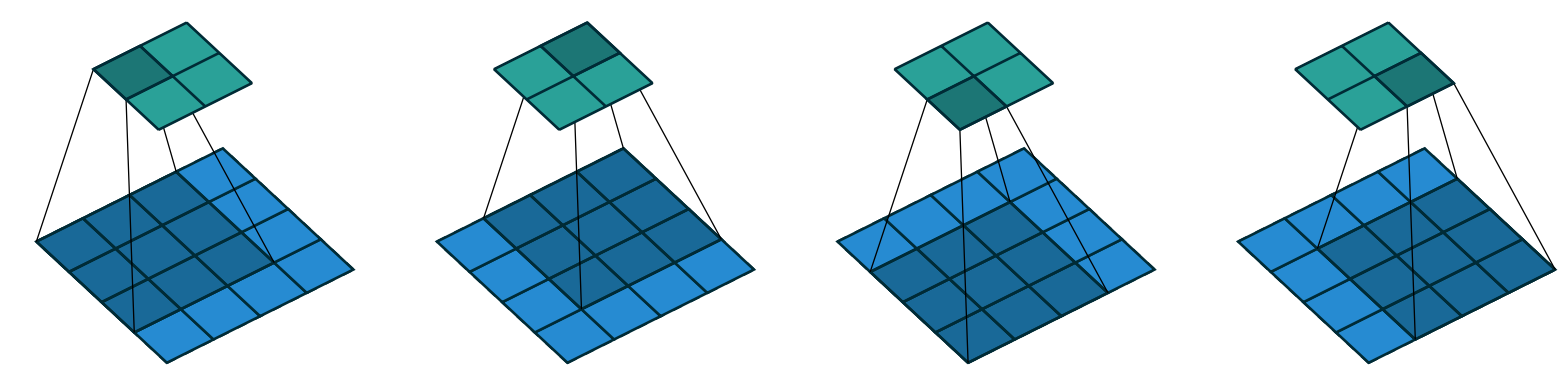
\includegraphics[width=\textwidth]{images/att_00028.png}
    }
    \caption{Depiction of how a convolution computes its outputs. A $4\times 4$ input convolved with a $3\times 3$ kernel produces a $2\times 2$ output. Since no padding is used this constitues a valid convolution. \href{https://fastai.github.io/fastbook2e/images/att_00028.png}{Image Source}}
    \label{fig:convolution}
\end{figure}

The example seen in Figure \ref*{fig:convolution} shows only one channel and a procedure that employs no padding, leaving the output smaller than the input (called a valid convolution). Other than valid convolutions, padding the input by $\lfloor\frac{k}{2}\rfloor$ or $k - 1$, where $k$ is the size of the kernel, leaves us with a \emph{same} (same size as input) or \emph{full} (larger than input) convolution. Additionally, in reality inputs to a layer often have many channels and the layer should be able to produce an arbitrary amount of output channels. In this case there exists a kernel $K_{\text{in}, \text{out}}$ for each combination of input channels $C_\text{in}$ and output channels $C_{\text{out}}$ whose convolution results are then added up for each output channel, so that
$$
    \text{out}_j = \sum_{k=1}^{C_\text{in}} K_{k,j} * \text{input}_k
$$
where $*$ is the convolution operation. There are other approaches to handle multi channel scenarios, but this is the simplest one and the one employed in the thesis. 

Using a convolution layer has several advantages over using fully connected layers. First of all is a reduction in \emph{learnable parameters} (see \ref*{sec:training}) which reduces computational resources required and thereby speeds up training. Secondly it introduces the inductive bias that positionally close data points are correlated and relevant to each other to the model, which is reasonable especially in tasks concerning computer vision. 

Imagine having a model that tries to detect circles in an image. It makes sense to assume that features which make up a circle are positionally close to each other. Convolutions are also translationally invariant, which in the same example means that for two identical circles at different locations in the input, the identical output is produced at their corresponing position, which is not the case for fully connected layers, where very different weights might me learned for different positions in the picture if data is insufficiently random.

Many architectures in the computer vision field now purely employ convolutional layers (\emph{fully convolutional neural networks}) or use very few fully connected layers only to compute the final output of the network at the end. 

There are additional constructs that can be used in neural networks, such as \emph{pooling} layers, which also move a kernel over the input like a convolution, but instead take the average or maximum of the covered elements as their output. As such, the pooling layer contains no variable parameters. They are generally used to reduce the dimensions of the feature map to further speed up training time and make the model more stable by promoting invariance to small perturbations in the input.
    \section{Semantic Image Segmentation}
\label{sec:imseg}

With the knowledge of how neural networks perform their computation in general we need to think about how a specific task can be accomplished by them.
To do this we need to find a specialized representation of the problem which networks can be applied to.

There are several common types of problems within computer vision that have different kinds of encodings for their solution space. As stated in the introduction, the task which this thesis is trying to solve lies in the category of \emph{Instance Segmentation}, but can be accomplished by instead doing \emph{Semantic Image Segmentation}.
For this task the network input is an image and the network is supposed to assign each pixel one of a predetermined set of \emph{classes} to which the pixel belongs to. For example in the case of the \emph{Cityscapes Dataset}\cite{cordtsCityscapesDatasetSemantic2016a}, the data consists of images of inner city traffic situations from the perspective of a car, and the classes are subjects like \emph{car}, \emph{road}, \emph{person}, \emph{building} etc.

\begin{figure}[htbp]
    \centering
    \begin{tabular}{ll}
        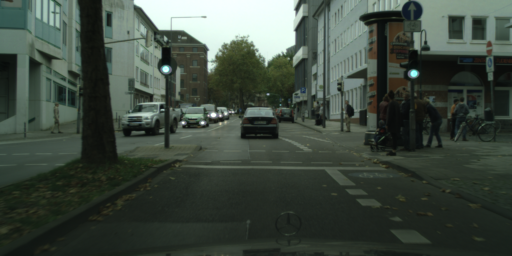
\includegraphics[width=0.45\textwidth]{images/aachen_000029_000019_leftImg8bit.png}
        &
        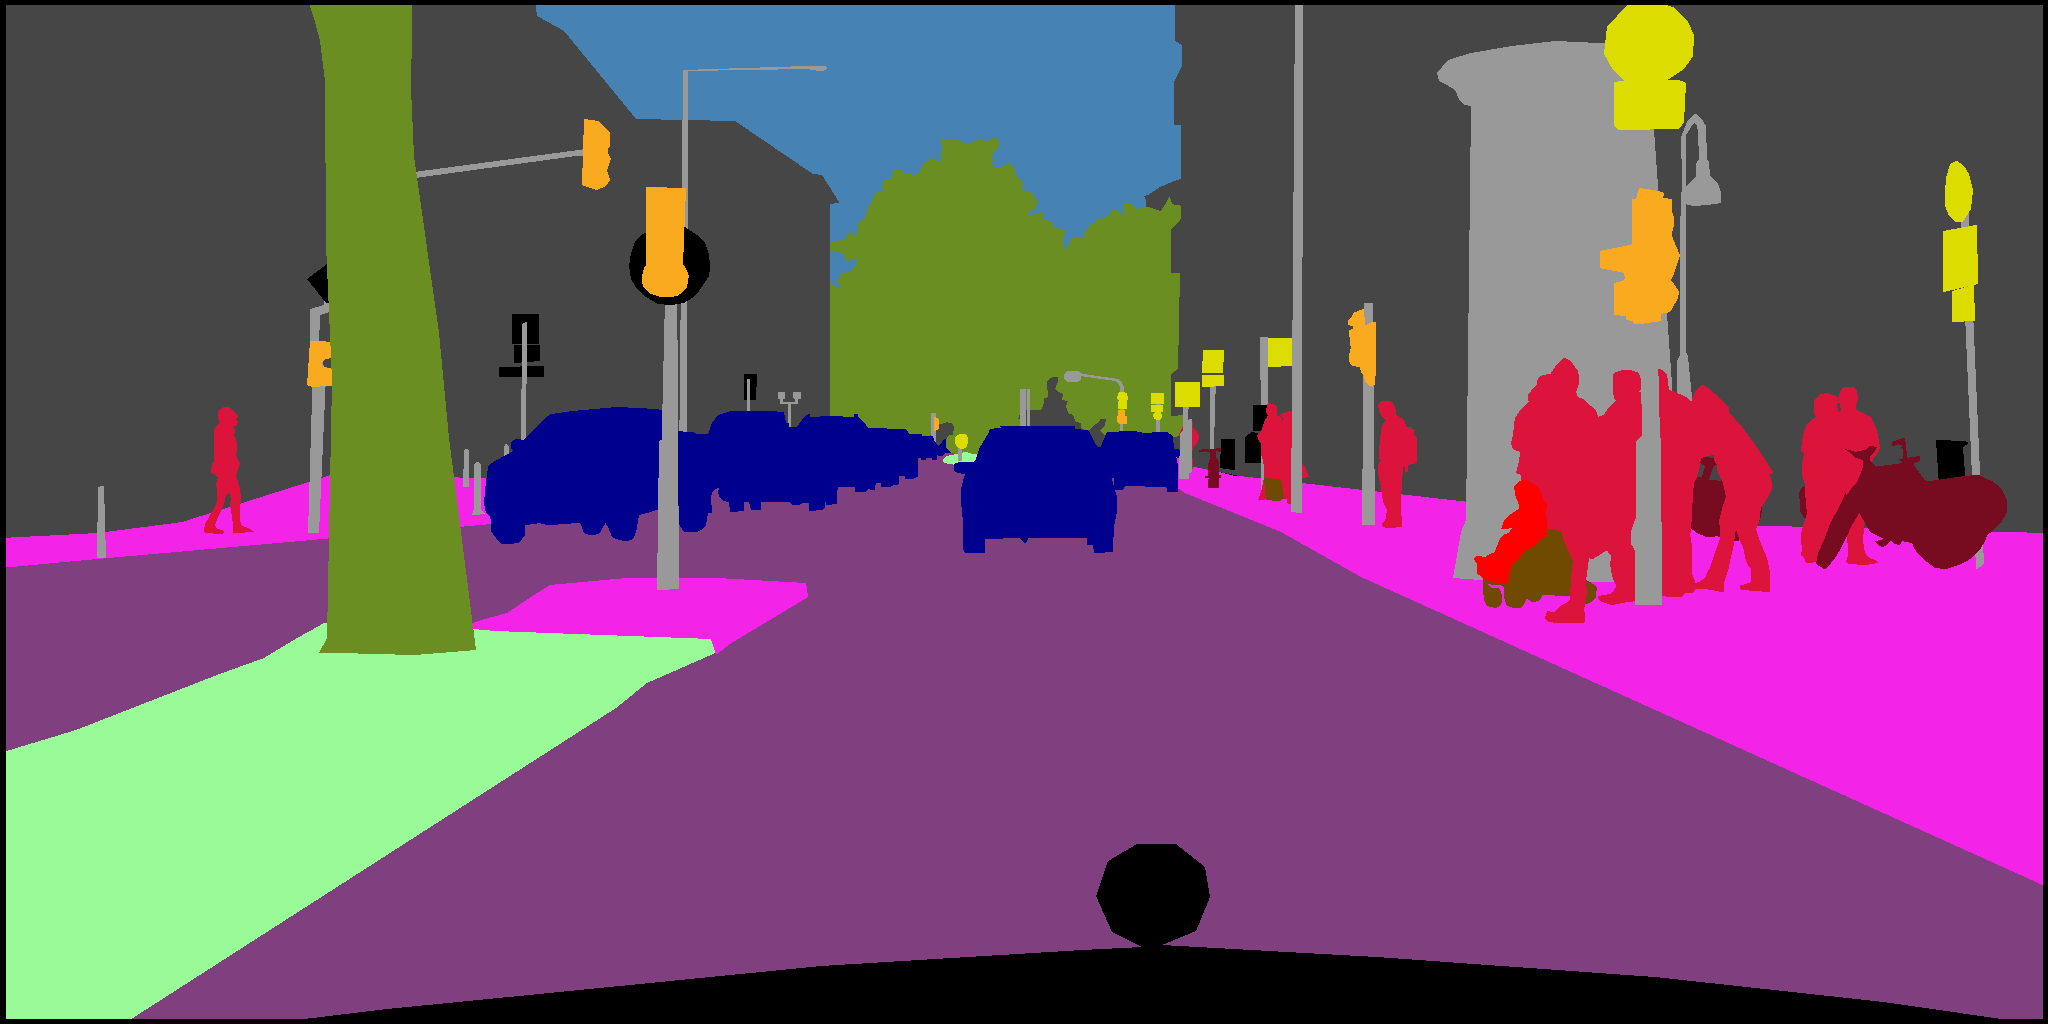
\includegraphics[width=0.45\textwidth]{images/aachen_000029_000019_gtFine_color.png}
    \end{tabular}
    \caption{A sample from the dataset \emph{Cityscapes}. On the left is the image that acts as an input for the network and on the right is the corresponding ground truth label mask showing different classes in different colors. \cite{cordtsCityscapesDatasetSemantic2016a}}
    \label{fig:cityscapes_smpl}
\end{figure}

A model for this task would now output a map $O\in\mathbf{R}^{C\times M\times N}$ with the same spatial dimensions as the image and a number of channels $C$ equivalent to the number of possible classes. Each output pixel consists of a vector $\mathbf{x}\in \mathbb{R}^C$ where each entry $x_i$ corresponds to how much the network thinks the pixel belongs to class $i$. The channel with the highest value is the class the network has classified the pixel as.

These outputs can now be normalized to probabilities by applying the \emph{softmax} function to them or converted to a segmentation mask by using the \emph{argmax} function.

To evaluate how well a network performs on the segmentation task, the \emph{Intersection over Union} (IoU) for each class is computed. For the set $A$ of pixels labeled as a certain class by the network and the set $B$ of pixels which are part of that class in the ground truth the IoU is defined as
$$
    \text{IoU} = \frac{\left|A\cap B \,\right|}{\left|A\cup B \,\right|}\quad .
$$
This metric is very informative to look at per class when trying to figure out specific strengths and weaknesses of the model, but typically the mean over all classes (mIoU) is used to evaluate the model as a whole.

A big challenge in developing machine learning solutions for this kind of task is its demand for varied data to train models on. High quality annotated data is very time and cost consuming to produce. 
For example according to the Cityscapes team, one annotated image such as seen in Figure \ref{fig:cityscapes_smpl} took \SI{90}{min} to create. 
Further in this thesis techniques to mitigate this problem and achieve good results on a small set of annotated data will be discussed.

    \section{Training neural networks}
\label{sec:training}

As mentioned previously neural networks with appropriate weights can be used to approximate any mathematical mapping between two Euclidean spaces (and more), but which weights are appropriate is not at all apparent for any nontrivial task. 
Similarly to how humans don't immediately perform at their potential best at a new task, but can train the brain to improve at solving a particular problem by strengthening the corresponding nervous pathways through repeated exercise, a neural network can \emph{learn} the correct weights for a task during \emph{neural network training}.

Training a neural network requires annotated data for a problem, where the ground truth for the problem at hand is known and encoded in a way that is compatible with the output format of the neural network. 
Keeping in line with the topic of this thesis, for a pixel level semantic segmentation task, this would be in the form of segmentation masks where each pixel has the id of the correct class as its value. 

Training happens in several steps. First, a sample from the training data is taken and the model, typically initialized with (semi-) random weights, computes its prediction for the problem (a segmentation mask). Then, a \emph{loss function} is applied to measure a distance between the prediction and the ground truth in the solution space. 
There are several functions which can be used as a loss function for one particular problem which may or may not perform better than others in expressing how wrong the model was with its prediction. 
Next, the gradient of the loss with regards to each learnable parameter is computed by using the chain rule for derivatives to propagate the error backwards through the network (\emph{backpropagation}). 
The parameters are then very slightly adjusted to reduce that error. 
There are several different rules for updating the weights with this gradient in each step, but widely used procedures include \emph{stochastic gradient descent (SGD)} and \emph{adam} \cite{kingmaAdamMethodStochastic2017}. 

There are several parameters that influence the progress of the training or even how the model operates, but aren't learnable parameters like the weights of the model. 
These parameters are called \emph{hyperparameters}. This includes the \emph{learning rate} which influences how much the parameters get updated in each step, but also things like the kernel size of a convolutional layer. 
Most of the time, samples aren't processed one by one, but stacked up in \emph{batches}, whose size (the \emph{batch size}) constitute another important hyperparameter. 
Processing multiple samples at once can be more efficient and also make the training process more stable by presenting more varied data to the network during each optimization step. However, batch size is limited by the size of the training samples in relation to the memory of the hardware used, so it can't be made arbitrarily large. 

Which hyperparameter values are used during training can have a huge impact performance, so finding optimal hyperparameters is vital when developing a model. 
The appropriate hyperparameters depend a lot on the training data and model architecture and are largely determined through trial and error. 
There are systematic approaches to hyperparameter tuning, but these are often very computationally expensive, since they perform a lot of trial runs. 
For simpler problems it is often enough to perform the search manually, by starting at values which are known to be in the correct order of magnitude for similar problems and then make informed adjustments based on the results of fewer trial runs. 

Another important part of model training is \emph{data augmentation}, which means to apply random perturbations to the inputs or even the model itself (in the case of \emph{dropouts}) during training to prevent the model from \emph{overfitting}. 
This refers to the model \emph{memorizing} the training data instead of learning the concept of the problem, leading to high performance on the training data at the cost of worse performance on unseen data, which is undesirable in most cases. 
The noise applied by augmentation reduces the likelihood of this happening and generally improves model performance. 
Since the augmentations are random, they functionally produce additional samples, which can help especially in cases with little training data. 
Some typical augmentations for computer vision tasks include \emph{random horizontal/vertical flipping}, \emph{scaling and resizing} or \emph{applying gaussian noise}. 

    \chapter{Architectures}
    \label{sec:architectures}
    When approaching a problem with a machine learning solution in mind, the first decision one has to deliberate on is the choice of network architecture used. 

In the case of neural networks, the word \emph{architecture} means which kind of layers are connected to each other in what order to produce the output of the network.

The landscape of machine learning architectures has become incredibly diverse, with improvements being made constantly.
With some architectures being better suited for certain problems or priorities, which architecture one chooses has a significant impact on the results.

In this section, an overview over the architectures used in the thesis and their main ideas will be given.
    \section{The U-Net}

The \emph{U-Net} is a network achitecture first proposed by \Citeauthor{ronnebergerUNetConvolutionalNetworks2015} in 2015 for application in biomedical segmentation tasks, for example segmenting cell borders in microscopic images of HeLa cells. 
The challenges the authors were facing at the time are similar to the ones in this thesis, where training data for biomedical segmentation tasks was scarce, which is why the U-Net was makes sense as a starting point for the problem of droplet segmentation.

It is a fully convolutional network, which were on the rise to surpass older state of the art neural networks for classification tasks at the time. 
The network employs an \emph{encoder-decoder} structure, meaning the architecture consists of a contracting path and a expanding path, the \emph{encoder} and \emph{decoder} respectively, as seen in Figure \ref{fig:unet}.

\begin{figure}[htbp]
    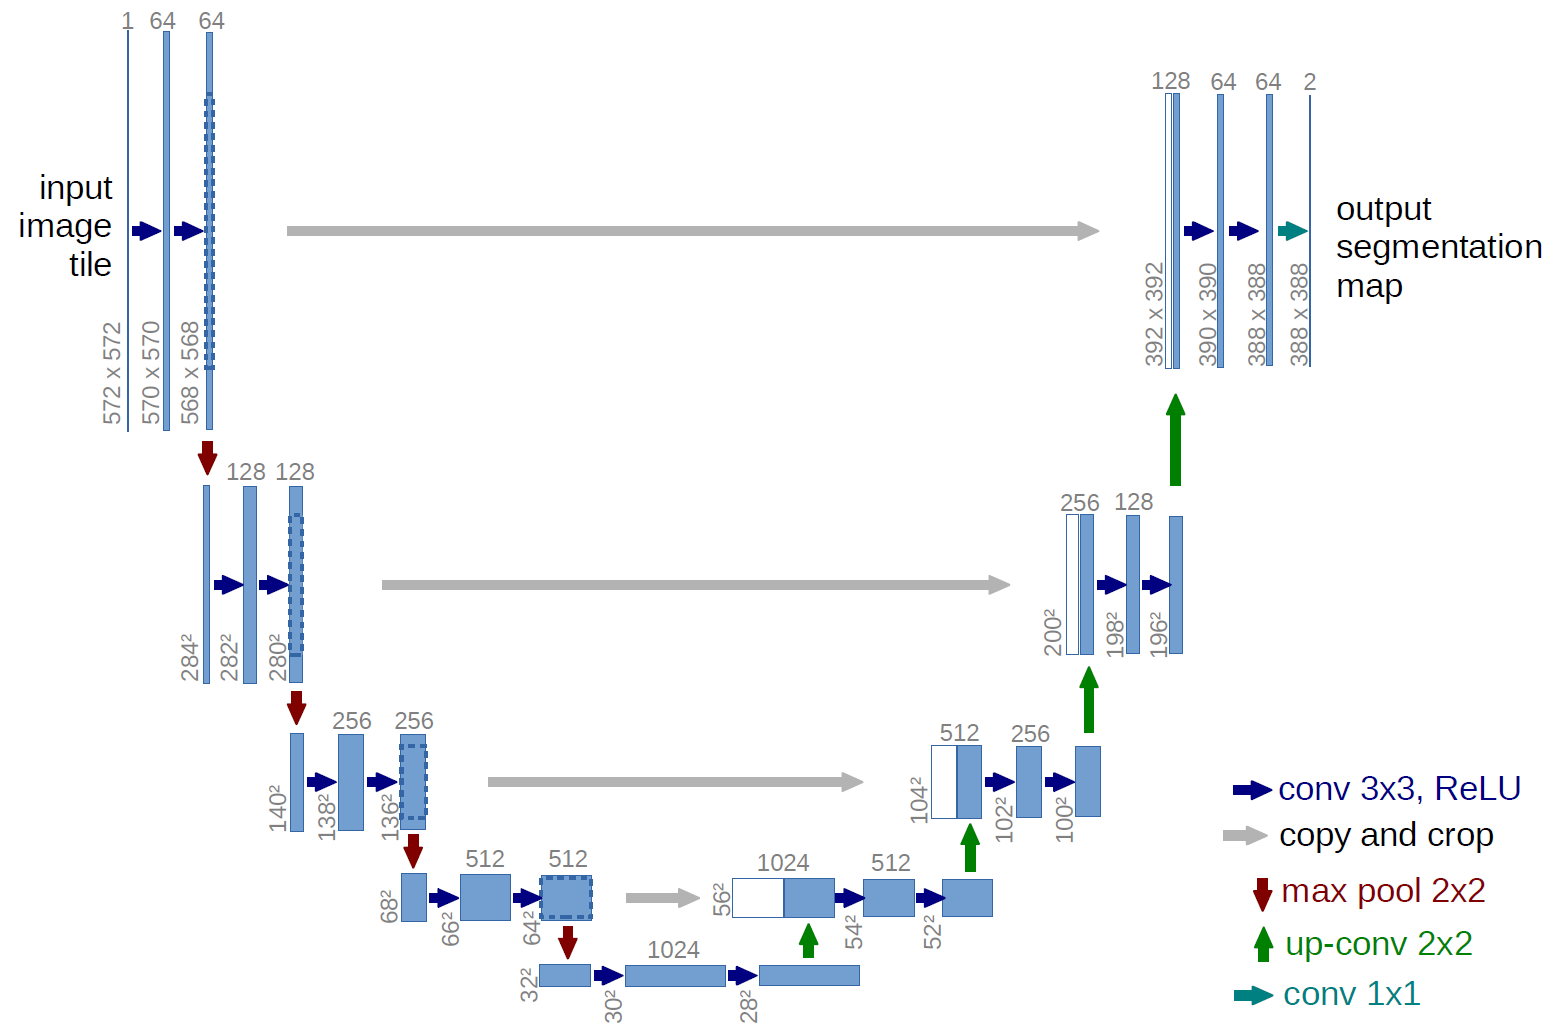
\includegraphics[width=\textwidth]{images/unet.png}
    \caption{The original U-Net architecture proposed in \cite{ronnebergerUNetConvolutionalNetworks2015}, for an example of a $572\times 572$ input, with the number of channels of the layer written above the blue boxes representing the feature map after each layer passthrough. The legend shows which operation was used between each feature map.}
    \label{fig:unet}
\end{figure}

The encoder path computes a number of features at four different spatial input sizes with two $3\times 3$ convolutions followed by a ReLu, which are then downsampled by a $2\times 2$ max-pooling layer. 
With each of these blocks, the spatial resolution is halfed along each axis, while the number of feature channels is doubled.

The features output by each block depend on different sized regions of the initial input. 

The values of blocks with high spatial resolution consider only small patches in the input image, while a lot of pixels influence each value for the lower blocks. 
The large \emph{perceptive field} of the lower blocks allow for rich contextual information to be encoded in their feature maps.

In a classification problem, such contracing networks would be used by feeding the highly dense information of the last encoder block to a few fully connected layers which make the final classification decision. 
In this case, since a classification for each pixel is needed, the encoded information must now be scaled back up to the desired resolution.

The decoder path is symmetrical to the encoder path, halving the number of feature channels in each block and upsampling the spatial resolution by using $2\times 2$ \emph{transposed convolutions}, which act like a backwards pass through a normal convolution.
After the last upsampling block a final $1\times 1$ convolution is used to decide the final class for each pixel.

However, as is, this structure has a key flaw when it comes to creating segmentation masks. While it is feasable to deduce general locations of objects from the highly contextual encoder features, it is difficult to infer their exact boundaries, because the spatial resolution has been compressed so much. 

This is where another key aspect of the U-Net architecture comes in. 
By concatenating the outputs of each encoder block to the input of their respective decoder block, we allow the decoder to not only utlize the context information provided by the last enocoder layers, but also the very localized features of the high resolution blocks.

This combination allows the U-Net to predict the correct classes along with their precise spatial location.

The U-Net outperformed its predecessors by a large margin and has since been developed further. Its concepts still serve as the basis for popular segmentation networks.\\

One way in which the original U-Net architecture is often modified, is using more sophisticated models for the encoder module, which is the approach taken in this thesis. 
Obtaining better features has proven itself to lead to better overall results, so investing more capability in the encoder structure is often a good idea. 

This also comes with the added benefit that pretrained weights for common feature extractors like the \emph{ResNet} (more in \ref{sec:resnet}) are readily available. 
    \section{The ResNet}
\label{sec:resnet}

The \emph{Residual Network (ResNet)} is a deep neural network architecture first introduced by \Citeauthor{heDeepResidualLearning2015}\cite{heDeepResidualLearning2015} in 2015, which addresses the seemingly paradoxical circumstance that adding more layers to a deep neural network would degrade its performance compared to a shallower network, even though the solution space of the shallower model is a subspace of its deeper counterpart. 

Working from the idea that adding more layers to a network should not produce a higher error, since the additional layers could potentially just learn identity mappings, the authors surmised that the problem lied with the difficulty for the optimization process to learn the underlying desired mapping for a set of layers if the ideal mapping is closer to an identity mapping than a zero mapping.

The solution to this, proposed by ResNet, is to utilize residual connections between the input and output of a layer group, by directly adding the input to the output. 
Instead of having to learn the desired output mapping $\mathcal{H}(x)$, the layers now have to fit the residual mapping $\mathcal{F}(x) := \mathcal{H}(x) - x$, which the authors argue is easier for the optimizer to do.

\begin{figure}[htbp]
    \makebox[\textwidth][c]{
        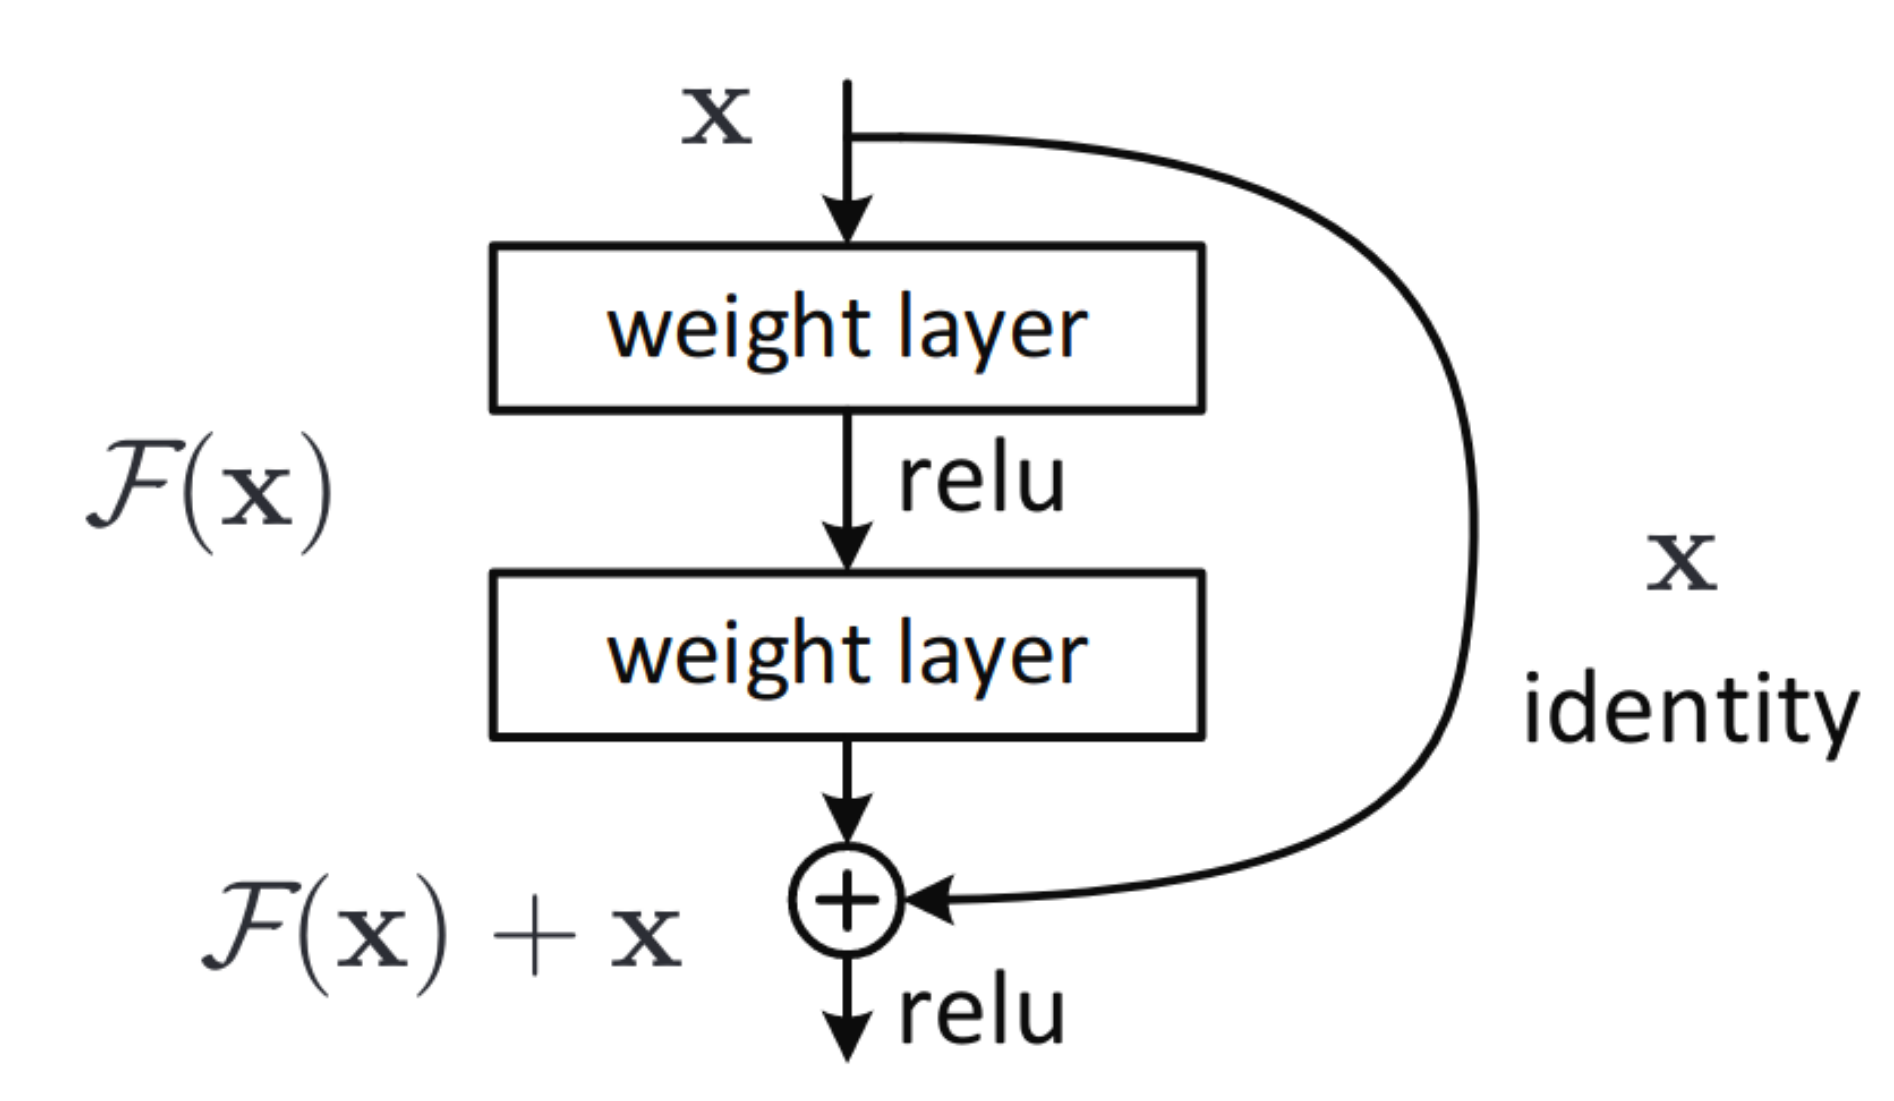
\includegraphics[width=0.4\textwidth]{images/Screenshot-20230207134546-1894x1101.png}
    }
    \caption{A depiction of a \emph{residual block} employed in the ResNet network architecture. The input of a group consisting of several layers is added directly to the output. The weighted layers can be linear layers but in practice, mostly convolutional layers are used. The blocks also consist of 3 layers the majority of the time. Image taken from \cite{heDeepResidualLearning2015}}
    \label{fig:resblock}
\end{figure}

Employing these \emph{residual blocks}, the convergence rate of the network is significantly improved, without adding any computational complexity. 
This enables the use of very deep networks, gaining substantial accuracy from the added layers.

Apart from the residual connections, the ResNet still follows a typical encoder architecture, with each block reducing spatial resolution, while increasing the number of feature channels.
There are several versions of the ResNet architecture, differing mainly by the number of layers used. 
\Citeauthor{heDeepResidualLearning2015} looks at networks with up to 152 layers (ResNet152), but deeper networks have been explored. 

Since the residual connection allow the network to propagate information from the shallower layers to the deeper layers more easily, it may also combat the problem of vanishing/exploding gradients, which were a challenge for increasingly deep models at the time, however the authors argue that this was already sufficiently addressed by regularization techniques such a \emph{Batch Normalization}. \cite{ioffeBatchNormalizationAccelerating2015}

ResNet was able to significantly outperform its state-the-art predecessors at the task of image classification and is widely used today, often as part of a larger model ensemble.

In this thesis, \emph{ResNet34 D} is used in most experiments, which makes several minor improvements over the regular ResNet.
This includes employing an average pooling layer before the strided $1\times 1$ convolution present in the identity path of each downsampling block to include all datapoints, switching the stride of convolutions in the residual path for the same reason and replacing the $7\times 7$ initial downsampling convolution with three $3\times 3$ convolutions.
These modifications see an improvement in classification error while only increasing computational cost slightly. \cite{heBagTricksImage2018} 

\begin{figure}[htbp]
    \makebox[\textwidth][c]{
        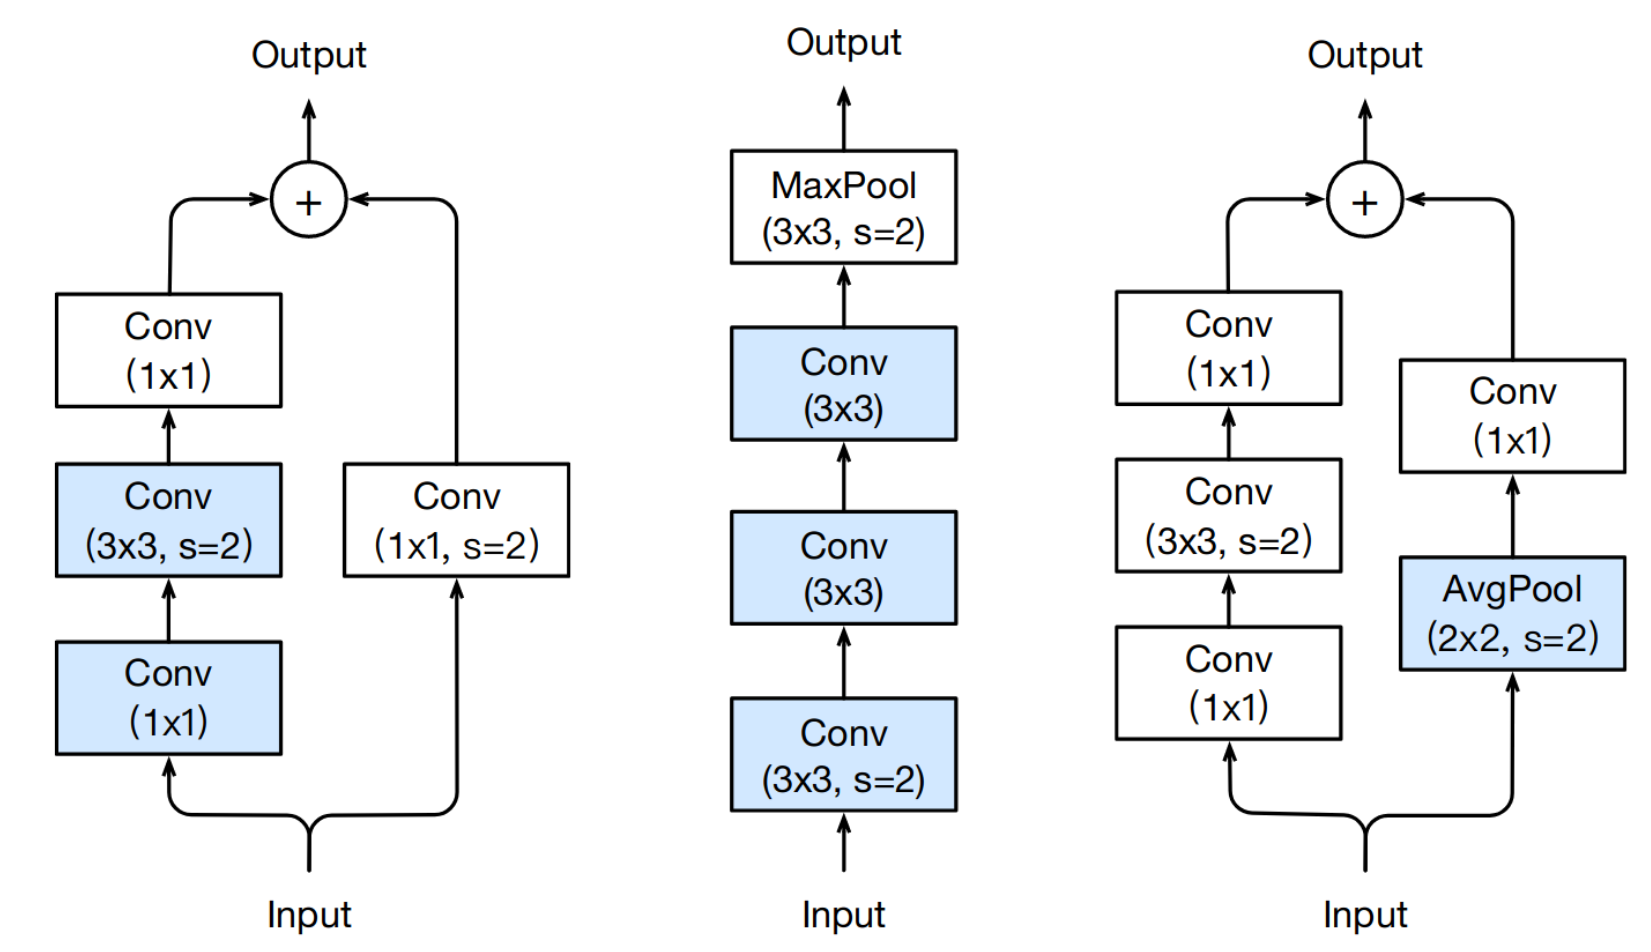
\includegraphics[width=0.9\textwidth]{images/Screenshot-20230207145624-1651x952.png}
    }
    \caption{Illustration of the three improvements made by ResNet34 D, with the blue boxes representing the changes made. Left depicts the change made to the residual path of the downsampling block, middle illustrates the changes made to the initial block of the network and right explains the changes to the identity path. $s$ represents the stride of the operations, with it being one if ommited. Image taken from \cite{heBagTricksImage2018}}
    \label{fig:resnet34d}
\end{figure}

\begin{figure}[htbp]
    \makebox[\textwidth][c]{
        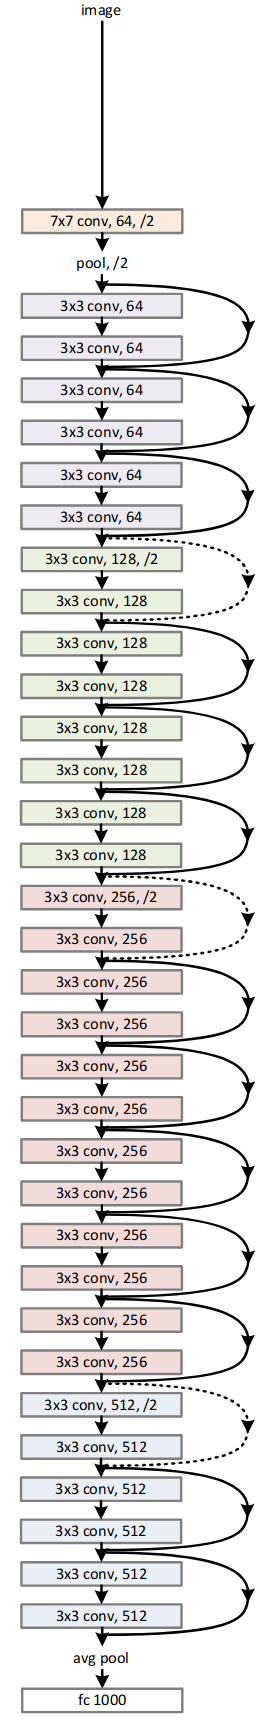
\includegraphics[width=0.2\textwidth]{images/Screenshot-20230207144959-265x1725.png}
    }
    \caption{Diagram for the ResNet34 model. Curved arrows represent a residual connection, with dotted arrows meaning the connection also downsamples the input. The four encoder blocks are colored differently. For use as an encoder, the fully connected layer at the end is omitted. Image taken from \cite{heDeepResidualLearning2015}}
    \label{fig:resnet34}
\end{figure}

    \chapter{Techniques used to improve model accuracy}
    \label{sec:techniques}
    Basic steps such as optimizing parameters for training are not the only methods available to try to improve the performance of the resulting model. 
Other techniques may be used to achieve better results, either by facilitating learning in some way or exploiting more data. 
In the following sections, the techniques employed during model development in this thesis will be explained more in depth.
    \section{Transfer Learning}
\label{sec:transfer_learning}

Coming back to the human learning analogy, it is often the case that knowledge or skills gained in one field can be applied to other fields, without having a lot of experience in these new disciplines. For example one might take their knowledge about composition from drawing to apply it to taking good pictures in photography. Although the technical details of both fields are different, they have some shared concepts, which help a person proficient in one to perform well in the other. That same person might also be able to improve in this new discipline faster than others, who do not have any applicable prior knowledge, because they can focus on learning other key skills needed to excel.

\emph{Transfer leaning} is the idea to apply this concept to neural network training. From a high level perspective, what happens during computation in a neural network, is that each layer transforms the input into an \emph{intermediate representation} of the data, which extracts different features present in the input. For example, one layer might learn to detect edges, which the next layer then combines to knowledge about the location of corners. As you can imagine, these types of features are useful for recognizing objects, such as a tennis ball, in a picture. It also stands to reason that these same features would be useful to detect circular droplets. The extracted features are rarely this clear cut or human-understandable as in this example, but the point remains the same. 

Using a model trained on one dataset and using these weights as a starting point to fine tune the model on the actual problem dataset is also called \emph{pretraining}. This is especially useful if the data for the target problem is scarce, as pretraining is often done on very large datasets such as \emph{ImageNet}\cite{dengImageNetLargescaleHierarchical2009}, which features over 14 million images (smaller subsets available) annotated for \emph{image classification}.
If the target problem is similar to the problem the model was pretrained on, the whole model can be used as a starting point for training. 
However, pretraining is also possible on a task different from the actual problem, in which case the pretrained model can only be used in a larger ensemble.

Pretrained weights for popular architectures are readily available for download and are employed in this thesis by using them as a feature extractor in an \emph{encoder-decoder} architecture (see section \ref{sec:architectures})

There are other forms of transfer learning, such as \emph{knowledge distillation}, where the concept is to use a complex model that is well adapted to the task to train a comparatively smaller model. The larger model has a higher knowledge capacity, but not all of this capacity has learned important knowledge. When training the smaller model on the soft outputs (before argmax) of the larger model, it may learn correlations which it might not have been able to learn on its own given its limited capacity. The smaller network could then be deployed instead of the larger one to save computation resources on weaker hardware.

In this thesis pretraining is used in two places. Firstly, for the encoder module of the U-Net architecture, a ResNet that is pretrained on the ImageNet dataset is used. Secondly, the experiments examine if pretraining the model on the Cityscapes dataset helps to improve performance on the vapour image dataset.
    \subsection{The mean teacher approach to semi supervised learning}
\label{sec:mean_teacher}

As mentioned multiple times already, the starting hurdle for building machine learning solutions is obtaining enough high quality annotated data. 
For image segmentation tasks, this means segmentation masks, which are notoriously time consuming to produce. 
In our case, no annotated data was present in the beginning and it would be unreasonable to spend a large amount of time to annotate a lot of images, so only a limited amount of labeled samples were produced. 
In contrast, unlabeled images can be obtained very quickly and in large amounts, as one good measurement run can produce hundreds to thousands of images (even though not all of them may be usable).

Thus it would be very beneficial if we could make use of this unlabeled data in some way during training. 
Approaches to learning that utilize both labeled and unlabeled data are called \emph{semi-supervised learning}, in contrast to \emph{(fully-)supervised} or \emph{unsupervised learning}, where only labeled or no labeled data is used respectively. 
One example for such a procedure is called the \emph{Mean Teacher approach}.\cite{tarvainenMeanTeachersAre2018}

The main idea of the Mean Teacher approach it to use two models, one \emph{student} and one \emph{teacher}, and have the student learn from examples produced by the teacher.

The reason unlabeled data is not directly usable for model training is that no classification cost can be applied to the outputs, as the target is undefined.
While there is no way to automatically generate a 100\% accurate target, as this is essentially what we try to train our model to do, when we look at it the other way around, we can use a model to approximate the target to a degree.
However, using the same model we want to train to simply approximate its own training samples would not provide any benefit.
Two steps are are used in the Mean Teacher method to still make use of these kinds of \emph{pseudolabels}.

As mentioned in \ref{sec:training}, augmentation and regularization techniques have the purpose of enabling the model to learn the concept of its target function more broadly, since small variances in the input should still produce a similar output. 
This can be applied not only when comparing the output of the model to the ground truth, but also when comparing the outputs of the model for the same input data, but different levels of noise. 
In a sense, if the model has properly learned the correct abstractions, its prediction should be similar, even if the input is slightly different.
What this means concreetly in this case, is that the method uses the teacher to make a prediction on an input without any noise and then computes student predicitons on the same input to which  augmentations have been applied.
In general, the teacher should have an easier time to predict accurate labels for a sample without noise, so a slightly better approximation of the theoretical correct labels should be produced. 
A \emph{consistency cost} can then be applied between student and teacher predictions which are then used in the same way as the \emph{classification cost} to update student weights.

Another way to improve the relative quality of the pseudolabels is to improve the teacher model they are generated by.
This is where the second key concept of the method comes in.
Instead of using the same weigths for both student and teacher models, the \emph{exponential moving average} (EMA) of the student weights are used for the teacher.
What this means is, if $\theta_t$ are the weights of the student at step $t$ and $\theta'_t$ are teacher weights at the same point, $\theta'_{t+1}$ is defined as follows:
$$
    \theta'_{t + 1} = \alpha\theta'_t + (1 - \alpha) \theta_t
$$
where $\alpha$ is a smoothing coefficient called the \emph{EMA decay}.

The EMA of a model has been observed to be slightly better than the model itself, as well as being more stable during the training process, since changes to the student model are only adapted slowly. Combining this with the noisy student inputs makes it possible to extract a lot of improvment from unlabeled examples, but can also be applied during training steps with labeled data. 

\begin{figure}[htbp]
   \makebox[\textwidth][c]{
        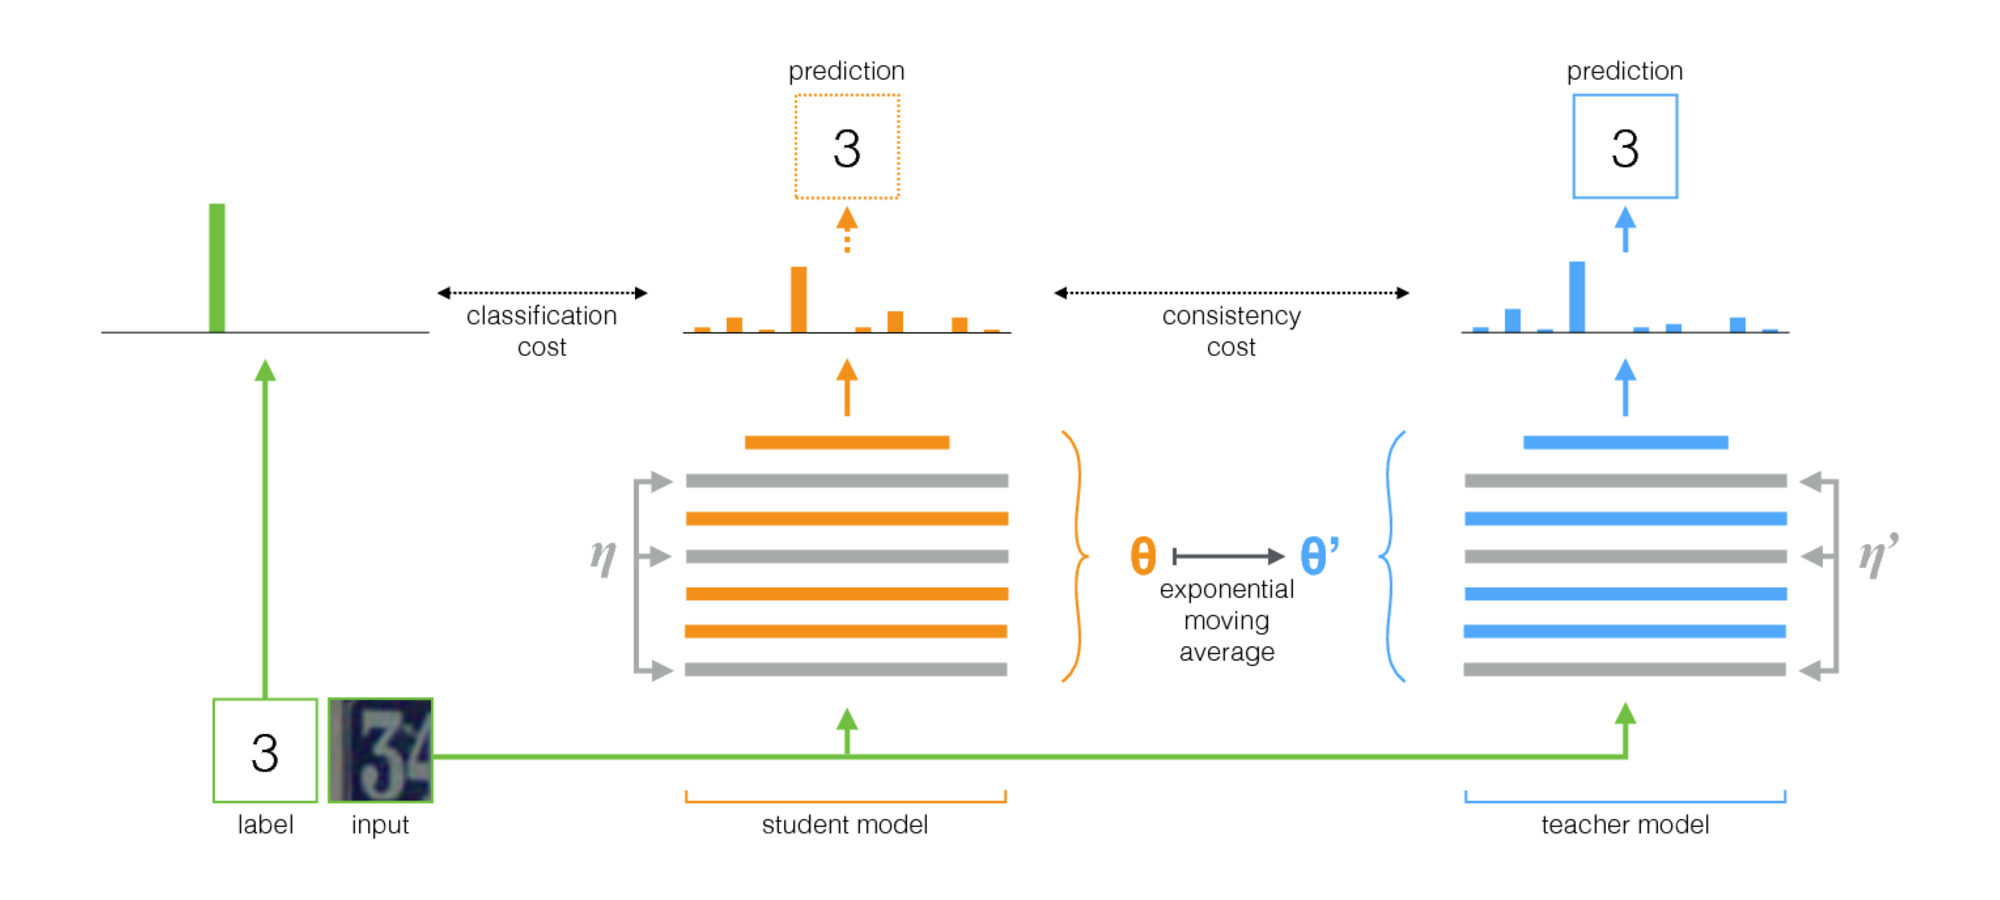
\includegraphics[width=\textwidth]{images/mean_teacher.png}
   }
   \caption{Schematic depiction of the Mean Teacher method. The graphic illustrates a single training step with one labeled sample for the image classification task. The classification loss is applied between the ground truth and the model predictions, while the consistency cost is computed between the soft outputs of both models. After updating the student weights, new teacher weights are computed as the EMA of the student weights. Steps with unlabeled samples simply omit the classification cost. Image taken from \cite{tarvainenMeanTeachersAre2018}}
   \label{fig:mean_teacher}
\end{figure}

During traing, it is necessary to apply a relative weight between classification loss and consistency loss, since initially, the teacher model may produce very bad outputs and which might also differ a lot from the student outputs, since no concepts haven been learned yet. 
If the consistency is given too much weight the model will prioritize being consistent with the teacher over predicting the correct classes for the labeled examples, potentially hurting or preventing any training progress. 
Thus, the weight of the consistency loss should start low and be slowly ramped up over the period of the training. 

Another key aspect of the method is considering which augmentations are chosen for the student inputs. To produce a large enough difference between outputs, strong augmentations are necessary to achieve the best improvements. The augmentations should also be well tailored to the dataset that is being trained on. 

Lastly, as mentioned above, the method introduces the hyperparameter $\alpha$ into the training, which has a big influence over the improvement that can be achieved. If it is too low, the benefits of using the EMA may not be present as much, since the teacher is too similar to the student. If it is too high, the teacher may not be updated quickly enough to incorporate the students improvement. 

The applicability of the mean teacher method will be more closely examined during the experiments of the thesis, with the goal to improve overall accuracy as well as generalization of the model produced. 

    \newpage 
%\nocite{*} 
\printbibliography[title={Bibliography}]

\end{document}